%%%%%%%%%%%%%%%%%%%%%%%%%%%%%%%%%%%%%%%%%
% Programming/Coding Assignment
% LaTeX Template
%
% This template has been downloaded from:
% http://www.latextemplates.com
%
% Original author:
% Ted Pavlic (http://www.tedpavlic.com)
%
% Note:
% The \lipsum[#] commands throughout this template generate dummy text
% to fill the template out. These commands should all be removed when
% writing assignment content.
%
% This template uses a Perl script as an example snippet of code, most other
% languages are also usable. Configure them in the "CODE INCLUSION
% CONFIGURATION" section.
%
%%%%%%%%%%%%%%%%%%%%%%%%%%%%%%%%%%%%%%%%%

%----------------------------------------------------------------------------------------
%	PACKAGES AND OTHER DOCUMENT CONFIGURATIONS
%----------------------------------------------------------------------------------------

\documentclass{article}

\usepackage{fancyhdr} % Required for custom headers
\usepackage{lastpage} % Required to determine the last page for the footer
\usepackage{extramarks} % Required for headers and footers
\usepackage[usenames,dvipsnames]{color} % Required for custom colors
\usepackage{graphicx} % Required to insert images
\usepackage{subcaption}
\usepackage{listings} % Required for insertion of code
\usepackage{courier} % Required for the courier font
\usepackage{lipsum} % Used for inserting dummy 'Lorem ipsum' text into the template

% Margins
\topmargin=-0.45in
\evensidemargin=0in
\oddsidemargin=0in
\textwidth=6.5in
\textheight=9.0in
\headsep=0.25in

\linespread{1.1} % Line spacing

% Set up the header and footer
\pagestyle{fancy}
\lhead{\hmwkAuthorName} % Top left header
\chead{\hmwkClass\ (\hmwkClassTime): \hmwkTitle} % Top center head
%\rhead{\firstxmark} % Top right header
\lfoot{\lastxmark} % Bottom left footer
\cfoot{} % Bottom center footer
\rfoot{Page\ \thepage\ of\ \protect\pageref{LastPage}} % Bottom right footer
\renewcommand\headrulewidth{0.4pt} % Size of the header rule
\renewcommand\footrulewidth{0.4pt} % Size of the footer rule

\setlength\parindent{0pt} % Removes all indentation from paragraphs

%----------------------------------------------------------------------------------------
%	CODE INCLUSION CONFIGURATION
%----------------------------------------------------------------------------------------

\definecolor{MyDarkGreen}{rgb}{0.0,0.4,0.0} % This is the color used for comments
\lstloadlanguages{Perl} % Load Perl syntax for listings, for a list of other languages supported see: ftp://ftp.tex.ac.uk/tex-archive/macros/latex/contrib/listings/listings.pdf
\lstset{language=Perl, % Use Perl in this example
	frame=single, % Single frame around code
	basicstyle=\small\ttfamily, % Use small true type font
	keywordstyle=[1]\color{Blue}\bf, % Perl functions bold and blue
	keywordstyle=[2]\color{Purple}, % Perl function arguments purple
	keywordstyle=[3]\color{Blue}\underbar, % Custom functions underlined and blue
	identifierstyle=, % Nothing special about identifiers
	commentstyle=\usefont{T1}{pcr}{m}{sl}\color{MyDarkGreen}\small, % Comments small dark green courier font
	stringstyle=\color{Purple}, % Strings are purple
	showstringspaces=false, % Don't put marks in string spaces
	tabsize=5, % 5 spaces per tab
	%
	% Put standard Perl functions not included in the default language here
	morekeywords={rand},
	%
	% Put Perl function parameters here
	morekeywords=[2]{on, off, interp},
	%
	% Put user defined functions here
	morekeywords=[3]{test},
	%
	morecomment=[l][\color{Blue}]{...}, % Line continuation (...) like blue comment
	numbers=left, % Line numbers on left
	firstnumber=1, % Line numbers start with line 1
	numberstyle=\tiny\color{Blue}, % Line numbers are blue and small
	stepnumber=5 % Line numbers go in steps of 5
}

% Creates a new command to include a perl script, the first parameter is the filename of the script (without .pl), the second parameter is the caption
\newcommand{\perlscript}[2]{
	\begin{itemize}
		\item[]\lstinputlisting[caption=#2,label=#1]{#1.pl}
	\end{itemize}
}

%----------------------------------------------------------------------------------------
%	DOCUMENT STRUCTURE COMMANDS
%	Skip this unless you know what you're doing
%----------------------------------------------------------------------------------------

% Header and footer for when a page split occurs within a problem environment
\newcommand{\enterProblemHeader}[1]{
	%\nobreak\extramarks{#1}{#1 continued on next page\ldots}\nobreak
	%\nobreak\extramarks{#1 (continued)}{#1 continued on next page\ldots}\nobreak
}

% Header and footer for when a page split occurs between problem environments
\newcommand{\exitProblemHeader}[1]{
	%\nobreak\extramarks{#1 (continued)}{#1 continued on next page\ldots}\nobreak
	%\nobreak\extramarks{#1}{}\nobreak
}

\setcounter{secnumdepth}{0} % Removes default section numbers
\newcounter{homeworkProblemCounter} % Creates a counter to keep track of the number of problems
\setcounter{homeworkProblemCounter}{-1}

\newcommand{\homeworkProblemName}{}
\newenvironment{homeworkProblem}[1][Problem \arabic{homeworkProblemCounter}]{ % Makes a new environment called homeworkProblem which takes 1 argument (custom name) but the default is "Problem #"
	\stepcounter{homeworkProblemCounter} % Increase counter for number of problems
	\renewcommand{\homeworkProblemName}{#1} % Assign \homeworkProblemName the name of the problem
	\section{\homeworkProblemName} % Make a section in the document with the custom problem count
	\enterProblemHeader{\homeworkProblemName} % Header and footer within the environment
}{
	\exitProblemHeader{\homeworkProblemName} % Header and footer after the environment
}

\newcommand{\problemAnswer}[1]{ % Defines the problem answer command with the content as the only argument
	\noindent\framebox[\columnwidth][c]{\begin{minipage}{0.98\columnwidth}#1\end{minipage}} % Makes the box around the problem answer and puts the content inside
}

\newcommand{\homeworkSectionName}{}
\newenvironment{homeworkSection}[1]{ % New environment for sections within homework problems, takes 1 argument - the name of the section
	\renewcommand{\homeworkSectionName}{#1} % Assign \homeworkSectionName to the name of the section from the environment argument
	\subsection{\homeworkSectionName} % Make a subsection with the custom name of the subsection
	\enterProblemHeader{\homeworkProblemName\ [\homeworkSectionName]} % Header and footer within the environment
}{
	\enterProblemHeader{\homeworkProblemName} % Header and footer after the environment
}

%----------------------------------------------------------------------------------------
%	NAME AND CLASS SECTION
%----------------------------------------------------------------------------------------

\newcommand{\hmwkTitle}{Project 4} % Assignment title
\newcommand{\hmwkDueDate}{Sunday,\ April\ 2,\ 2018} % Due date
\newcommand{\hmwkClass}{CSC411} % Course/class
\newcommand{\hmwkClassTime}{L0101} % Class/lecture time
\newcommand{\hmwkAuthorName}{Ying Yang} % Your name

%----------------------------------------------------------------------------------------
%	TITLE PAGE
%----------------------------------------------------------------------------------------

\title{
	\vspace{2in}
	\textmd{\textbf{\hmwkClass:\ \hmwkTitle}}\\
	\normalsize\vspace{0.1in}\small{Due\ on\ \hmwkDueDate}\\
	\vspace{0.1in}
	\vspace{3in}
}

\author{\textbf{\hmwkAuthorName}}
%\date{} % Insert date here if you want it to appear below your name

%----------------------------------------------------------------------------------------

\begin{document}

	\maketitle
	\clearpage
	%----------------------------------------------------------------------------------------
	%	PROBLEM 1
	%----------------------------------------------------------------------------------------

	% To have just one problem per page, simply put a \clearpage after each problem

	\begin{homeworkProblem}[ Part 1]

		\noindent \textit{Environment}
		
		$\newline$
		The grid is represented by horizontal, vertical and diagonal indices. The coordinates are the indices from 0 - 8. The win-set is represented by a fix matrix in which the first row represents 3 sets of horizontal rows for which a player wins the game, the second row represent the vertical column, and the third row represents the diagonal of the tictactoe. 
        
        The attributes turn represents whose turn to play the game (player1 or player 2). The attribute done means whether the game is over (when a player wins, or a tie occurs).
        
        Play a game of TicTacToe by calling the step(), and render() methods.
        
        \begin{lstlisting}[language=Python, caption=Compute network function]
      	env.step(0)
      	(array([1, 0, 0, 0, 0, 0, 0, 0, 0]), 'valid', False)
      	env.render()
      	x..
      	...
      	...
      	====
      	env.step(2)
      	(array([1, 0, 2, 0, 0, 0, 0, 0, 0]), 'valid', False)
      	env.render()
      	x.o
      	...
      	...
      	====
      	env.step(4)
      	(array([1, 0, 2, 0, 1, 0, 0, 0, 0]), 'valid', False)
      	env.render()
      	x.o
      	.x.
      	...
      	====
      	env.step(8)
      	(array([1, 0, 2, 0, 1, 0, 0, 0, 2]), 'valid', False)
      	env.render()
      	x.o
      	.x.
      	..o
      	====
      	env.step(6)
      	(array([1, 0, 2, 0, 1, 0, 1, 0, 2]), 'valid', False)
      	env.render()
      	x.o
      	.x.
      	x.o
      	====
      	env.step(1)
      	(array([1, 2, 2, 0, 1, 0, 1, 0, 2]), 'valid', False)
      	env.render()
      	xoo
      	.x.
      	x.o
      	====
      	env.step(3)
      	(array([1, 2, 2, 1, 1, 0, 1, 0, 2]), 'win', True)
      	env.render()
      	xoo
      	xx.
      	x.o
      	====
        \end{lstlisting}
        

	\end{homeworkProblem}
	\clearpage
	%----------------------------------------------------------------------------------------
	%	PROBLEM 2
	%----------------------------------------------------------------------------------------

	\begin{homeworkProblem}[ Part 2]

		\noindent \textit{Complete the implementation so that policy is a neural network with one hidden layer}
			
		$\newline$
		

		\begin{homeworkProblem}[ Part 2 (a)]
				\begin{lstlisting}[language=Python, caption=Policy implementation]
			class Policy(nn.Module):
			"""
			The Tic-Tac-Toe Policy
			"""
			def __init__(self, input_size=27, hidden_size=64, output_size=9):
			super(Policy, self).__init__()
			# TODO
			self.linear_f1 = nn.Linear(input_size, hidden_size)
			self.linear_f2 = nn.Linear(hidden_size, output_size)
			
			def forward(self, x):
			# TODO
			h = F.relu(self.linear_f1(x))
			out = F.softmax(self.linear_f2(h))
			return out
			\end{lstlisting}
		\end{homeworkProblem}
	
	
		\begin{homeworkProblem}[ Part 2 (b)]
			\begin{lstlisting}[language=Python, caption=Policy]
			policy = Policy()
			state = np.array([1,0,1,2,1,0,1,0,1])
			state = torch.from_numpy(state).long().unsqueeze(0)
			state = torch.zeros(3,9).scatter_(0, state, 1).view(1, 27)
			print(state)
			\end{lstlisting}
			
			\begin{lstlisting}[language=Python, caption=output]
			Columns 0 to 12 
			0     1     0     0     0     1     0     1     0     1     0     1     0
			
			Columns 13 to 25 
			1     0     1     0     1     0     0     0     1     0     0     0     0
			
			Columns 26 to 26 
			0
			[torch.FloatTensor of size 1x27]
			\end{lstlisting}
			State what each of the 27 dimensions mean.
			
			The 27 dimensions is formatted as a 3 X 9 matrix.
			
			Each column index represents the position of grid.
			
		\end{homeworkProblem}
	
		\begin{homeworkProblem}[ Part 2 (c)]
			Explain what the value in each dimension means.
			The values in each dimension are the probabilities of the agent's next move to that position. 
			
			The policy is stochastic since the agent uses a random policy to make its next move.
		\end{homeworkProblem}
	\end{homeworkProblem}
	\clearpage
	%----------------------------------------------------------------------------------------
	%	PROBLEM 3
	%----------------------------------------------------------------------------------------

	\begin{homeworkProblem}[Part 3]

		\begin{homeworkProblem}[Part 3a]
			\noindent \textit{Implement the compute\_returns function}
			$\newline$
			\begin{lstlisting}[language=Python, caption=output]
			l = len(rewards)
			rewards = np.array(rewards)
			gammas = np.array([gamma ** (i) for i in range(l)])
			
			G = []
			for i in range(l):
				G.append(sum(rewards[i:] * gammas[:l - i]))
			return G
			\end{lstlisting}

		\end{homeworkProblem}

		\begin{homeworkProblem}[Part 3b]
			\noindent \textit{Explain why can we not update weights in the middle of an episode}\\
			
			When we are in the middle of the episode, we haven't yet finished computing the final result for reward. As a result, if we compute backward pass before we got the reward result, we could get inaccurate result, since if we compute the gradient based on inaccurate number. Therefore, we should update the weights after the episode.
			
		\end{homeworkProblem}

	\end{homeworkProblem}
	\clearpage

	%----------------------------------------------------------------------------------------
	%	PROBLEM 4
	%----------------------------------------------------------------------------------------

	\begin{homeworkProblem}[Part 4]
		
		\begin{homeworkProblem}[Part 4(a)]
			\begin{lstlisting}[language=Python, caption=modified function]
			def get_reward(status):
			"""Returns a numeric given an environment status."""
			return {
			Environment.STATUS_VALID_MOVE: 1,
			Environment.STATUS_INVALID_MOVE: -25,
			Environment.STATUS_WIN: 50,
			Environment.STATUS_TIE: 0,
			Environment.STATUS_LOSE: -50
			}[status]
			\end{lstlisting}
		\end{homeworkProblem}
		
		\begin{homeworkProblem}[Part 4(b)]
			\noindent \textit{Explain the choices that you made in 4(a)}\\
			
			The environments status were given weight based on the principle of rewarding biggest on win and penalize biggest on lose. In the same way, reward on status that contribute to valid moves and penalize on status that contribute to invalid moves. As a result, valid move is considered as a good move, and was given a positive number: 1. The invalid move is bad, so it should be penalized, and it was given: -25. The win status should be rewarded big, so it was given a big positive number: 50. The tie status is given 0 since it doesn't contribute to win or lose. Finally, the lose status was given  -50 to get penalized. 
			
		\end{homeworkProblem}
	
	\end{homeworkProblem}
	\clearpage

	%----------------------------------------------------------------------------------------
	%	PROBLEM 5
	%----------------------------------------------------------------------------------------

	\begin{homeworkProblem}[Part 5]

		\begin{homeworkProblem}[Part 5a]
			
		Plot the training curve of the tictactoe model.
		
		Hidden units = 64 units
		
		\begin{figure*}[h!]
			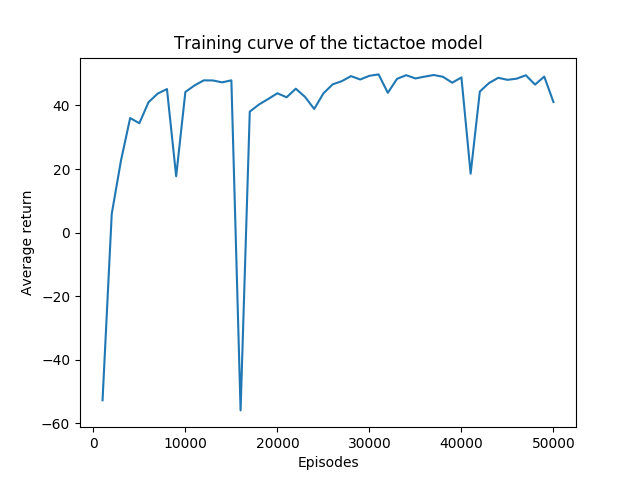
\includegraphics[scale=1]{part5a_hidden64.png}
			\caption{training curve of the tictactoe model, with 64 hidden units}
			\label{fig:randim}
		\end{figure*}	
			
		\end{homeworkProblem}
		
		\clearpage
		
		\begin{homeworkProblem}[Part 5b]
			
			Plot the training curve of the tictactoe model, by tuning the hyperparameter hidden units with 3 different values.
		
		1. Hidden units = 16 units
		
		\begin{figure*}[h!]
			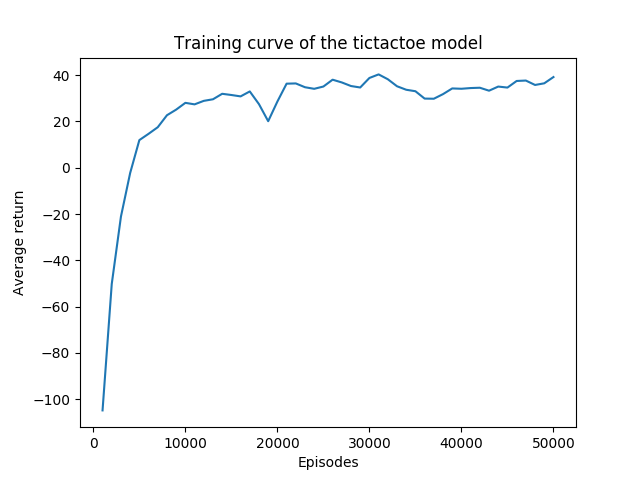
\includegraphics[scale=0.7]{part5b_hidden16.png}
			\caption{training curve of the tictactoe model, with 16 hidden units}
			\label{fig:randim}
		\end{figure*}	
	
	   2. Hidden units = 32 units
	   
	   \begin{figure*}[h!]
	   	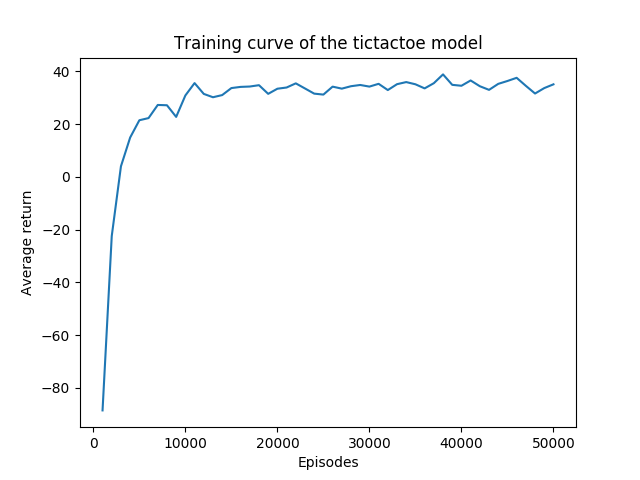
\includegraphics[scale=0.7]{part5b_hidden32.png}
	   	\caption{training curve of the tictactoe model, with 32 hidden units}
	   	\label{fig:randim}
	   \end{figure*}	
		
		3. Hidden units = 128 units
		
		\begin{figure*}[h!]
			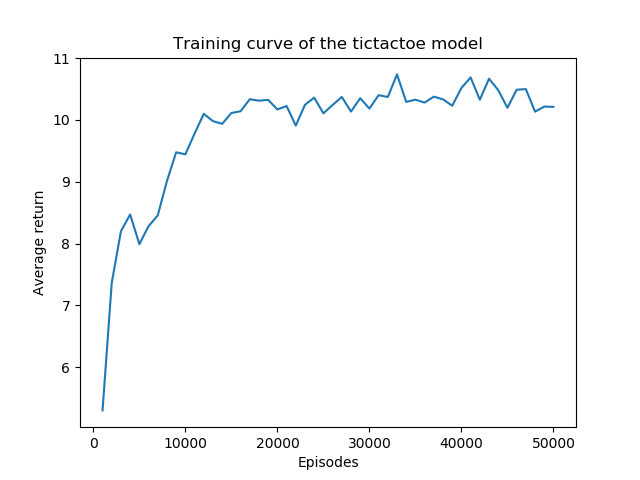
\includegraphics[scale=0.7]{part5b_hidden128.png}
			\caption{training curve of the tictactoe model, with 128 hidden units}
			\label{fig:randim}
		\end{figure*}
		
			4. Hidden units = 256 units
			
			\begin{figure*}[h!]
				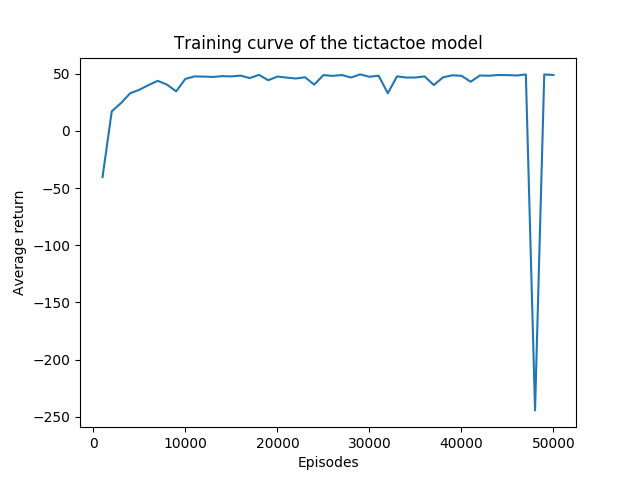
\includegraphics[scale=0.7]{part5b_hidden256.png}
				\caption{training curve of the tictactoe model, with 256 hidden units}
				\label{fig:randim}
			\end{figure*}
		
		After experimenting with 3 different number of hidden units : 16, 32, 128 and 256, it was possible to observe that the hyperparameter setting to 256s gave the best results. For hidden units 16 and 32, the average return was below 40, for 128, the average return was varying in the 40s and for 256, the average return almost reached 50.
		
		\end{homeworkProblem}

		\begin{homeworkProblem}[Part 5c]
			
		One of the first things that your policy should learn is to stop playing invalid moves. At around what episode did your agent learn that? State how you got the answer.
		
		The agent learned to stop playing invalid moves at around 4000th iteration. This can be observed by counting the number of invalid moves for 100 random games. By inspecting the result, starting at 3000th iteration, the number of invalid moves dramatically decreased 
		from 126 invalid moves to only 27 invalid moves. 
		
		\end{homeworkProblem}
	
		\begin{homeworkProblem}[Part 5d]
			\noindent \textit{Use your learned policy to play 100 games against random. }\\
		
			How many did your agent win / lose / tie? 
		
			Results for playing 100 games against random
			
			wins: 96        losses: 3       ties:1
			
			Display five games that your trained agent plays against the random policy. 
			\begin{lstlisting}[language=Python, caption=modified function]
			Game 1
			...
			.x.
			o..
			====
			..o
			.xx
			o..
			====
			..o
			xxx
			o..
			====
			wins: 1 losses: 0       ties:0
			
			Game 2
			...
			.xo
			...
			====
			...
			.xo
			xo.
			====
			..x
			.xo
			xo.
			====
			wins: 1 losses: 0       ties:0
			
			Game 3
			..o
			.x.
			...
			====
			..o
			.xx
			o..
			====
			..o
			xxx
			o..
			====
			wins: 1 losses: 0       ties:0
			
			Game 4
			...
			.x.
			..o
			====
			.o.
			.x.
			x.o
			====
			.ox
			.x.
			x.o
			====
			wins: 1 losses: 0       ties:0
			
			Game 5
			.o.
			.x.
			...
			====
			.o.
			.x.
			xo.
			====
			.ox
			.x.
			xo.
			====
			wins: 1 losses: 0       ties:0
			\end{lstlisting}
			
			Explain any strategies that you think your agent has learned.\\	
			
			By examining the steps that agent made, it is possible to see that the agent might learned to prioritize to make the step that allows to win the game fastest. For example, if it makes a first move without having the opponent blocking one of its winning lines (vertical, horizontal, diagonal), it will continue making move towards that line until the opponent blocks it. 
			
			Also, it might learned to avoid making useless moves such as making a move that doesn't block the opponent, or making a move that is obviously a dead move, that is useless. (such case figure below: )
			
			before : 
			
			o . . 
			
			x . o
			
			.  . .
			
			After : 
			
			o . . 
			
			x x o
			
			.  . .
			
			Finally, it always starts by picking the middle of the board, and this might be a learned strategy to more easily win the game.
			
			
		\end{homeworkProblem}
	\end{homeworkProblem}
	\clearpage
	%----------------------------------------------------------------------------------------
	%	PROBLEM 6
	%----------------------------------------------------------------------------------------

	\begin{homeworkProblem}[Part 6]

		\begin{homeworkProblem}[Part 6a]
		\noindent \textit{Use the model checkpoints saved throughout training to explore how the win / lose / tie rate changed throughout training}
		
		Graph of win/lose/tie rate changed throughout the training
		\begin{figure*}[h!]
			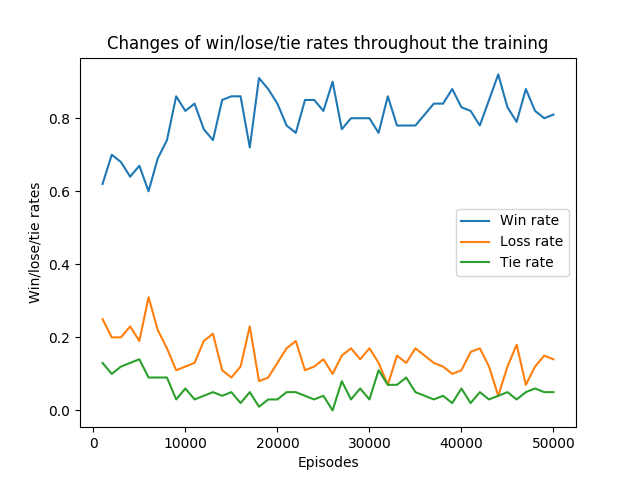
\includegraphics[scale=0.7]{part6.png}
			\caption{win/lose/tie rate changed throughout the training}
			\label{fig:randim}
		\end{figure*}	
		
		From the graph, we can see that the  win rate improved from around 62\% to around 81\%. Meanwhile, the lose rate and tie rate decreased from around 23\% to 15\%., 13\% to 5\% respectively. This shows that the agents has learned to make moves that rewards it for winning the game. 
		
		\end{homeworkProblem}


	\end{homeworkProblem}

	\clearpage
	%----------------------------------------------------------------------------------------
	%	PROBLEM 7
	%----------------------------------------------------------------------------------------
	
	 
	\begin{homeworkProblem}[Part 7]
		
		From the graphs, it is possible to observe that the probabilities for making first moves in cells 1, 2, 4, 5 were higher. As the model is trained more and more and the agent learned to win, the probabilities were higher for cells 3, 7 and 9, which makes sense. From the game play in part 6, it was observed that the agent always make the first move in the cell 5, and this is shown in the distribution where cell 5 got the highest probability compared to 1, 2 and 4. As a result, the model makes sense. 
		
		
		
	\begin{figure*}[!h]
		\begin{subfigure}{.35\textwidth}
			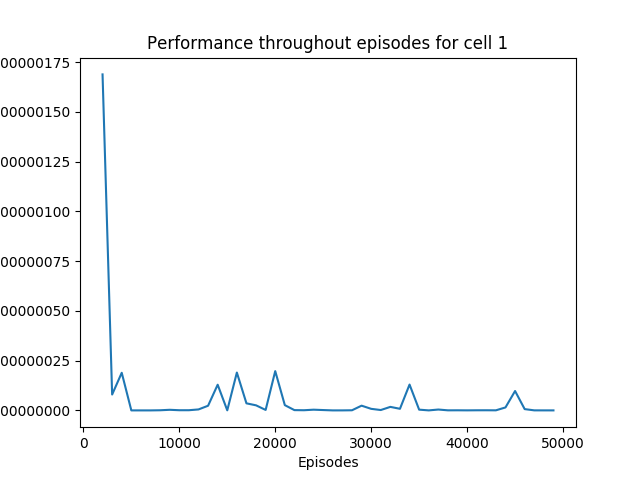
\includegraphics[width=1\linewidth]{part7_distribution_1.png}
			\caption{Cell 1}
		\end{subfigure}
		\begin{subfigure}{.35\textwidth}
			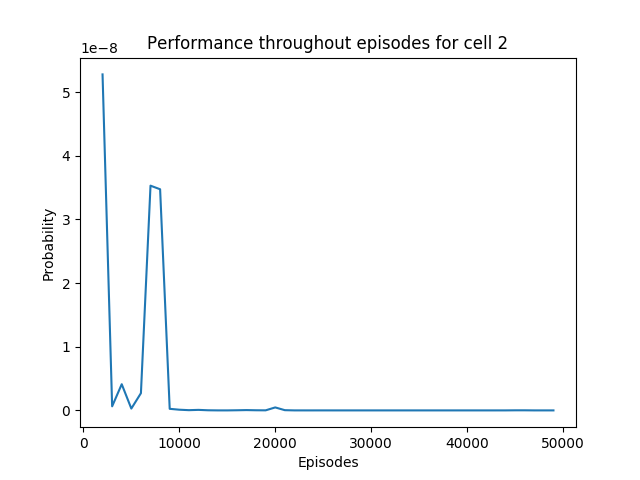
\includegraphics[width=1\linewidth]{part7_distribution_2.png}
			\caption{Cell 2}
		\end{subfigure}
		\begin{subfigure}{.35\textwidth}
			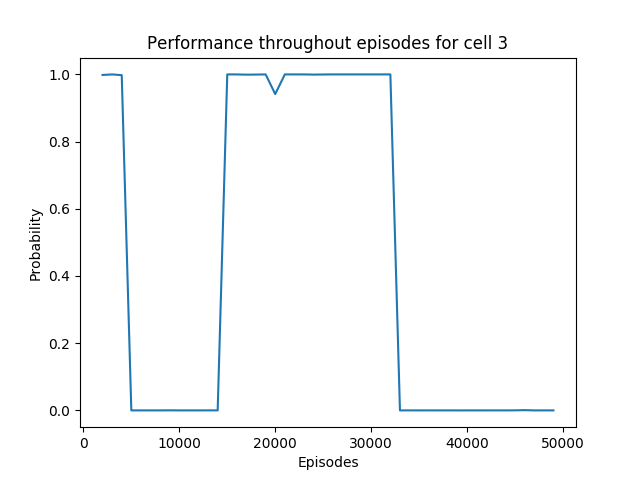
\includegraphics[width=1\linewidth]{part7_distribution_3.png}
			\caption{Cell 3}%
		\end{subfigure}
		\begin{subfigure}{.35\textwidth}
			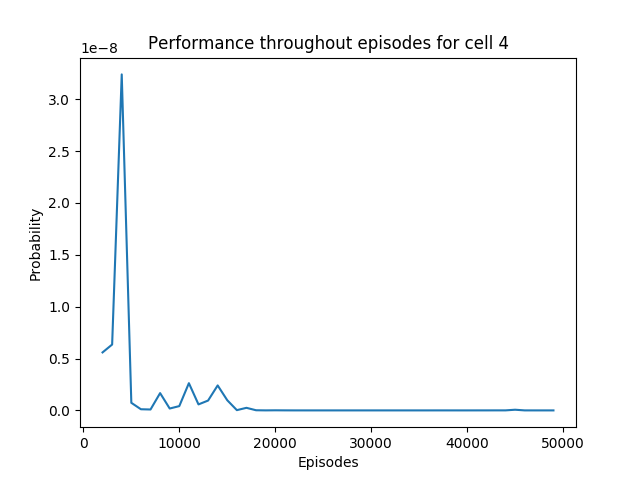
\includegraphics[width=1\linewidth]{part7_distribution_4.png}
			\caption{Cell 4}
		\end{subfigure}
		\begin{subfigure}{.35\textwidth}
			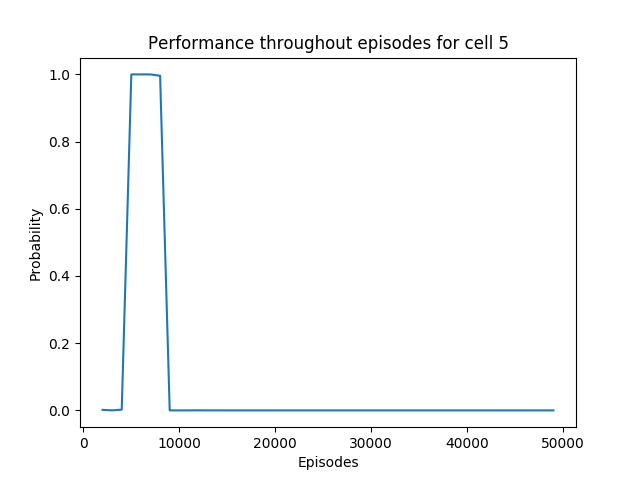
\includegraphics[width=1\linewidth]{part7_distribution_5.png}
			\caption{Cell 5}%
		\end{subfigure}
		\begin{subfigure}{.35\textwidth}
			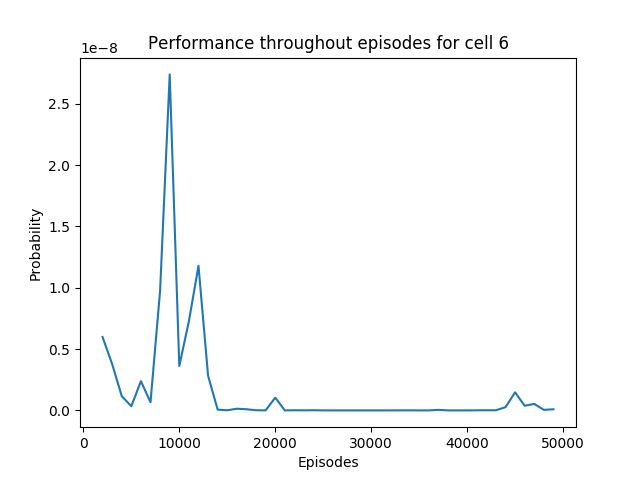
\includegraphics[width=1\linewidth]{part7_distribution_6.png}
			\caption{Cell 6}%
		\end{subfigure}
		\begin{subfigure}{.35\textwidth}
			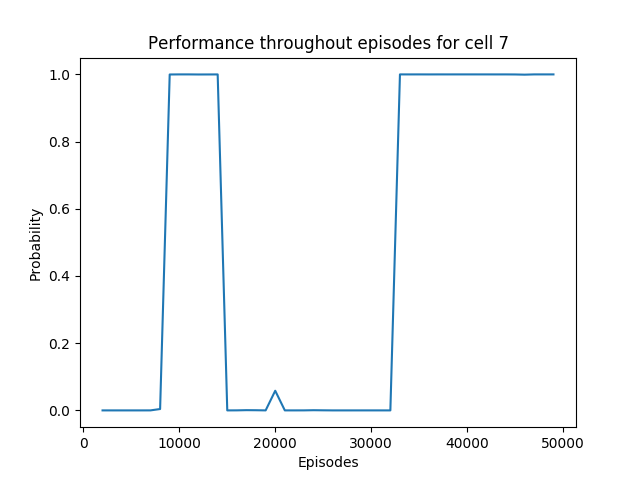
\includegraphics[width=1\linewidth]{part7_distribution_7.png}
			\caption{Cell 7}
		\end{subfigure}
		\begin{subfigure}{.35\textwidth}
			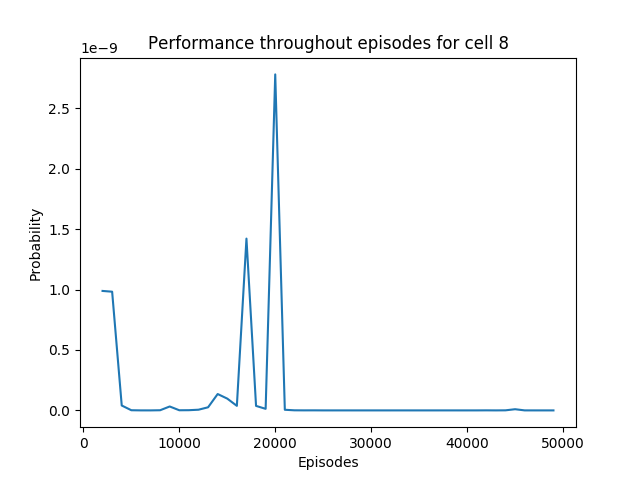
\includegraphics[width=1\linewidth]{part7_distribution_8.png}
			\caption{Cell 8}
		\end{subfigure}
		\begin{subfigure}{.35\textwidth}
			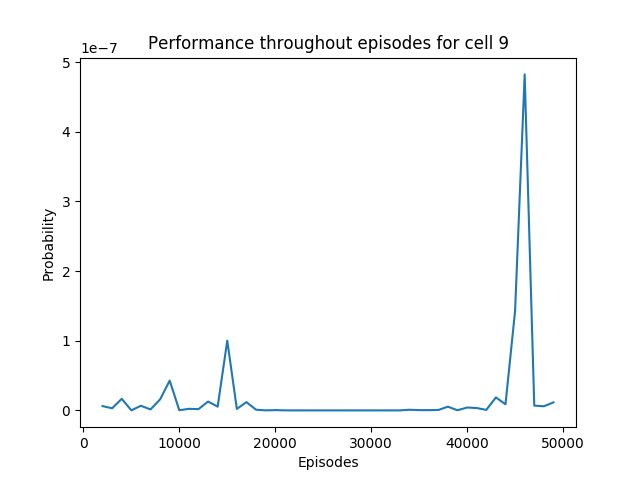
\includegraphics[width=1\linewidth]{part7_distribution_9.png}
			\caption{Cell 9}
		\end{subfigure}
		\caption{Display the weights}
		\label{Display the weights}
	\end{figure*}
	
	\end{homeworkProblem}

	\clearpage
	%----------------------------------------------------------------------------------------
	%	PROBLEM 7
	%----------------------------------------------------------------------------------------

	\begin{homeworkProblem}[Part 8]
	Your learned policy should do fairly well against a random policy, but may not win consistently. What are some of the mistakes that your agent made?
	
	Examples of mistakes that the agent made were it didn't prevent the opponent from winning by making random moves when the opponent had two same placements already. 
    
	\end{homeworkProblem}
	%----------------------------------------------------------------------------------------

\end{document}